\documentclass[12pt,a4paper,oneside]{memoir}
\usepackage{polski}
\usepackage[top=2.5cm, bottom=2.5cm, left=3.5cm, right=1cm]{geometry}
\usepackage{amsmath}
\usepackage{amsfonts}
\usepackage{amssymb}
\usepackage{graphicx}
\usepackage{titling}
\usepackage{titlesec}
\usepackage{fontspec}
\usepackage{siunitx}
\usepackage{caption}
\usepackage[
bookmarks=false,
pdfpagelabels=false,
hyperfootnotes=false,
hyperindex=false,
pageanchor=false,
hidelinks
]{hyperref}
\renewcommand{\chaptername}{} % Usunięcie napisu "Rozdział"
\sisetup{math-micro=\text{µ},text-micro=µ} % Konwersja znaku mikro z matematyki na tekst
\newfontfamily{\tytulyrozdzialow}{Arial} % Ustawienie czcionki Arial 
\setmainfont{Times New Roman} % Czionka TMR dla całego tekstu
\titleformat
	{\chapter} % Formatowanie rozdziałów
	[hang] % Tekst obok liczby
	{\fontsize{14pt}{16pt}\bfseries\tytulyrozdzialow\flushleftright} % Regulacja czcionki rozdziałów
	{\chaptertitlename\ \thechapter.} % Ustawianie wyglądu nagłówków rozdziałów
	{15pt} % Odstęp między liczbą a tekstem
	{} 
\setsecheadstyle{\fontsize{13pt}{15pt}\tytulyrozdzialow\bfseries} % Ustawienie stylu dla sekcji
\begin{document}
\renewcommand{\maketitle}
{
	\centering
	
\includegraphics[scale=0.1]{images/logo.jpg}\par\vspace{1cm}
	{\scshape\LARGE Kierunek: Elektronika i Telekomunikacja\\ Specjalność: Teleinformatyka \par}
	\vspace{1cm}
	{\scshape\Large Praca dyplomowa inżynierska\par}
	\vspace{1.5cm}
	{\huge\bfseries Stacja meteorologiczna oparta o ESP8266\par}
	\vspace{2cm}
	{\Large\itshape Damian Zaręba\\Nr albumu 8389\par}
	\vfill
	Promotor:\par
	dr inż. Tadeusz Leszczyński
	\vfill
	
	% Dół strony
	{\large Mława 2019r. \par}
}
\maketitle
\thispagestyle{empty}
\newpage
{\tytulyrozdzialow \tableofcontents}
\newpage
\flushleftright
\chapter{Wstęp}
	\hspace{\parindent} Założeniem pracy jest stworzenie stacji meteorologicznej opartej o mikroprocesor ESP8266, złożonej z kilku modułów. Tymi elementami są:
	\begin{itemize}{}{}
		\item Płyta główna z mikrokontrolerem ESP8266EX dla przetwarzania informacji z sensorów oraz sterowania zasilaniem całego urządzenia;
		\item Samodzielnie wykonany anemometr ultradźwiękowy do pomiaru kierunku i prędkości wiatru ze względów na koszty, ponieważ gotowe są zbyt drogie w stosunku do reszty;
		\item Sensor firmy BOSCH o nazwie BME280, który służy do odczytu temperatury, ciśnienia i wilgotności powietrza;
		\item Sensor firmy PLANTOWER o nazwie PMS7003, który mierzy ilość pyłu zawieszonego w powietrzu, o wielkości PM1.0, PM2.5 oraz PM10, mierzone w \si\micro g/m$^{3}$.
	\end{itemize}
	\par Jednym z elementów pracy jest schemat blokowy urządzenia oraz ogólny opis poszczególnych modułów wykorzystanych do zbudowania tego urządzenia, wliczając w to charakterystyki głównych komponentów dla każdego modułu. Udokumentowane zostanie m.in. skonfigurowanie środowiska, które zostały wykorzystane do stworzenia tego projektu.
	\par Następnie przejdę do analizy schematu urządzenia, a konkretnie płyty głównej, bazy z mikroprocesorami i zasilaniem dla wykorzystanych sensorów. Poddana dokładnej analizie będzie każda z części schematu, takie jak sekcja zasilania czy połączeniowa między płytą główną a sensorami.
	\par W kolejnym etapie pracy przedstawię kod źródłowy do wykorzystanego mikroprocesora. Dokładnie go omówię, wraz z algorytmami użytymi do jego napisania. Wykonuje on wiele zadań, m.in. odczytuje dane z sensorów czy kontroluje układy zasilania poszczególnych części.
	\par W przedostatnim punkcie przedstawię krótko projekt anemometru ultradźwiękowego służącego do pomiaru prędkości i kierunku wiatru. Omówiony zostanie schemat blokowy urządzenia i jego elektryczna reprezentacja.
	\par Ostatnim elementem projektu będzie ukazanie działania stacji. Pokażę to na przykładzie zdjęć sprzętu oraz zrzutów ekranu z aplikacji Blynk, służącej do interakcji z urządzeniem.

\chapter{Elementy składowe projektu} 
\section{ESP8266EX}
ESP8266EX to mikroukład z pełnym stosem TCP/IP oraz mikrokontrolerem wyprodukowanym przez Espressif w Szanghaju, Chiny.\\
Istnieje jego odmiana o nazwie ESP8285 z 1 MiB wbudowanej pamięci typu flash, co umożliwiało wykorzystanie go jako pojedynczego układu zdolnego do podłączenia się do sieci Wi-Fi, po podłączeniu zasilania. W odróżnieniu od rodziny mikrokontrolerów AVR nie może być zasilany napięciem 5V, jedynie 3.3 wolta.\\
\begin{figure}[h]
	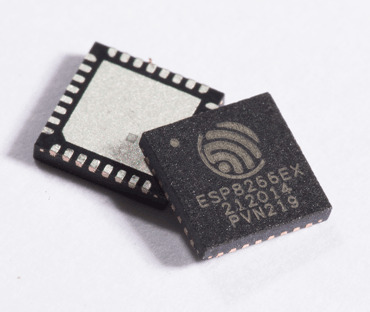
\includegraphics[scale=0.5]{images/esp8266ex.jpg}
	{\tytulyrozdzialow \footnotesize \caption[ESP8266EX]{Zdjęcie przedstawiające układ ESP8266EX}}
	\caption*{\textit{Źródło:\url{http://www.alphamicrowireless.com/media/562039/esp8266ex_370px.gif}}}
\end{figure}\\
ESP8266 posiada 32 bitowy procesor oparty o rdzeń Xtensa Diamond Standard 106Micro (LX106) firmy Tensillica o nominalnej wartości zegara wynoszącym 80 MHz oraz charakteryzuje się następującymi funkcjami:
\begin{itemize}
	\item 16 pinów GPIO
	\item SPI
	\item I$^2$C (programowa implementacja)
	\item I$^2$S z funkcją Direct Memory Access (współdzieli piny z GPIO)
	\item UART na wyznaczonych pinach GPIO oraz dodatkowy UART na GPIO2 służący jedynie do wysyłania danych
	\item 10-bitowy ADC oparty o sukcesywną aproksymację.
	\item Wbudowana obsługa Wi-Fi o standardach b/g/n według IEEE 802.11 z wbudowanym przełącznikiem TR,LNA,Balunem, wzmacniaczem mocy oraz siecią dopasowującą oraz możliwością podłączenia się lub tworzenia sieci z zabezpieczeniami WEP lub WPA/WPA2
\end{itemize}
Pamięć ulotna tego mikrokontrolera jest podzielona w następujący sposób:
\begin{itemize}
	\item 32 KiB RAM dla instrukcji
	\item 32 KiB RAM typu cache dla instrukcji
	\item 80 KiB RAM dla danych użytkownika
	\item 16 KiB RAM typu ETS dla danych "systemowych"
\end{itemize}
Obsługuje pamięć nieulotną typu flash po protokole SPI do pojemności 16 MiB, choć zazwyczaj korzysta się z pamięci o rozmiarach 512 KiB lub 4 MiB.\\
\begin{figure}[h]
	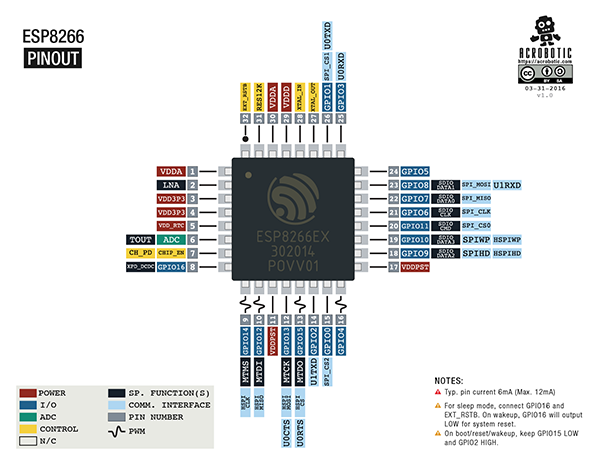
\includegraphics[scale=1.5]{images/esp8266_pinout.png}
	{\tytulyrozdzialow \footnotesize \caption[ESP8266EX]{Zdjęcie przedstawiające wyprowadzenia układu ESP8266EX}}
	\caption*{\textit{Źródło:\url{https://learn.acrobotic.com/uploads/esp8266_pinout.png}}}
\end{figure}\\
\newpage
\section{BME280}
\newpage
\chapter{Wykorzystane protokoły komunikacyjne}
\newpage
\chapter{Schemat funkcjonalny}

\newpage
\chapter{Schemat elektryczny}

\newpage
\chapter{Kod źródłowy} 

\newpage
\chapter{Opis anemometru} 

\newpage
\chapter{Infografika} 

\newpage
\listoffigures
\newpage
\listoftables
\newpage
\chapter{Spis załączników} 

\newpage
\chapter{Bibliografia}
 
\newpage
\chapter{Streszczenie} 

\end{document}